% !TEX root = ../../../main.tex
% 来源：中学数学实验教材·第一册（代数）
% 章节：因式分解与余式定理 / 余式定理及其推论
% 原始文件：5.tex，行 1071-1079
% 类型：tikz
% ---
    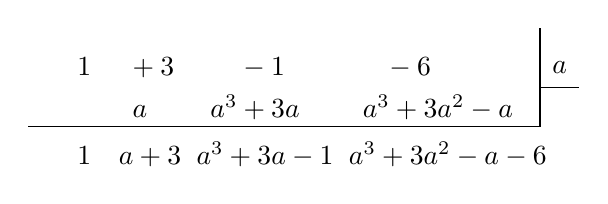
\begin{tikzpicture}
    \node at (0,0.5) [right] {$1\;\quad +3\;\qquad  -1\;\;\quad\quad\quad  -6$};
    \node at (0,0) [right] {$\qquad  a\; \quad \quad a^3+3a\;\quad\quad  a^3+3a^2-a$};
    \node at (0,-0.6) [right] {$1\quad  a+3\;\; a^3+3a-1\;\; \boxed{a^3+3a^2-a-6}$};
    \draw (-.5,-.25)--(6,-.25)--(6,1);
    \draw (6,.25)--(6.5,.25);
    \node at (6.25,.5){$a$};
    
    \end{tikzpicture}
